% !TEX root =  GroupDet.tex
\section{Introduction}

Social interactions are common, but they rarely take place in isolation. Conversations and other group interactions occur on busy streets, in crowded cafes, in large conference halls, and in other types of social gatherings. In these situations, before a computer vision system can \emph{recognize} distinctive group interactions, it must first \emph{detect} them by distinguishing between participants and by-standers, and by localizing these participants in space and time. This paper addresses this spatio-temporal detection problem for cases in which the actors in a large gathering can be approximately detected and tracked.

\begin{figure}[t]
\begin{center}
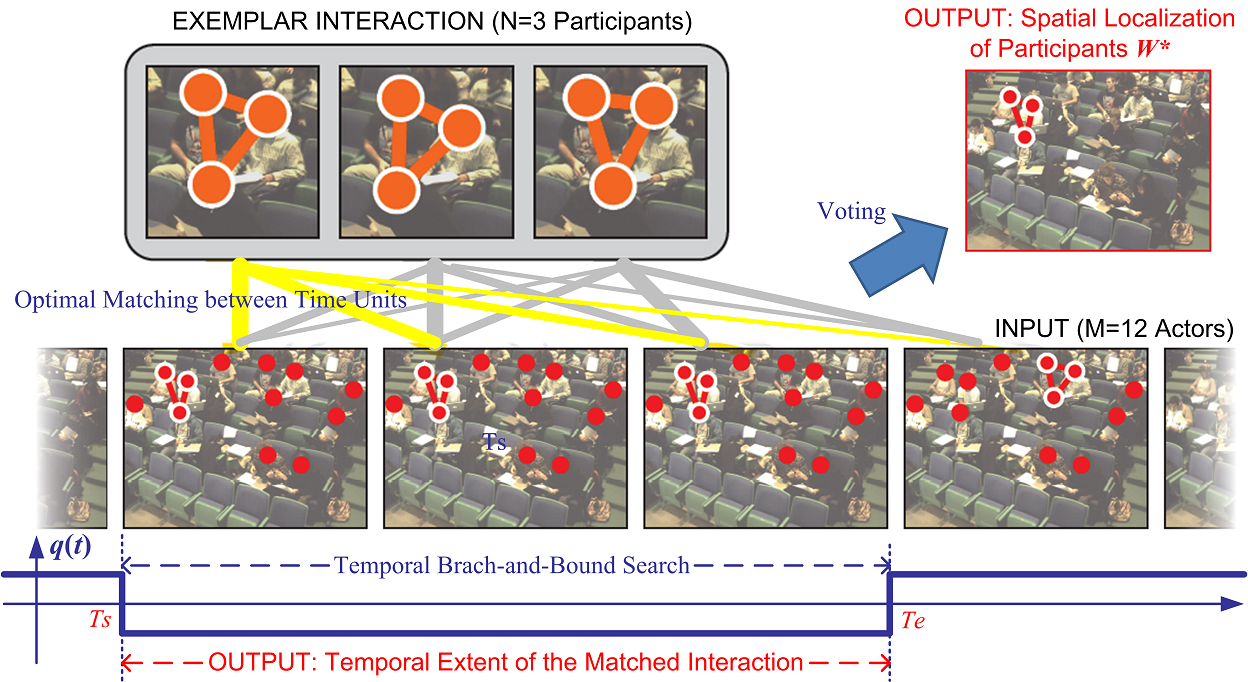
\includegraphics[width=\columnwidth]{diagram2.png}
\end{center}
\caption{Detecting and localizing interactions in social clutter. Given an exemplar video of an $N$-person social interaction, we seek to find similar interactions in a long input video with $M>N$ approximately-tracked actors. For each temporal frame in the exemplar, the $N$ best-matching participants are identified separately in each input video frame, and the matches are assigned scores. Matching scores are accumulated over time through Hough voting that is insensitive to tracking errors and changes in action rates, and this produces a spatial localization of the $N$ participating actors. Their interaction is then localized in time using an efficient branch-and-bound search.}
\label{diagram}
\end{figure}



We consider group interactions to be distinctive co-occurences of individual activities in space and time. When these take place within the context of a larger social gathering, we refer to those involved in an interaction as the \emph{participants} and the remaining others as the \emph{bystanders} with respect to that interaction. Our goal is to find participants among the bystanders; infer the beginning and end of the participants' interaction; and to ``recognize'' their interaction by matching it to a gallery of exemplars and (optionally) providing a class label. We consider the problem quite broadly, and we imagine that group interactions can be found in many places and at many times-scales. We might want to find in a video of a cocktail party all conversations that include three people with one person dominating the conversation for a sustained period of time. On a busy street corner, we could search for all cases in which two passersby exchange a simple greeting like ``hello.'' In a round-table discussion, we could seek intervals in which one speaker holds the attention of her neighbors for some extended time. In a collection of hockey games, we might want all instances of a ``three-on-one''. And in nature we might be interested in localizing instances of distinctive group interactions among populations of animals, insects, or bacteria. Each of these cases would likely require distinct algorithms for detecting and tracking the actors, and each would benefit from action descriptors that are tuned for that setting. But beyond this, each case can be abstracted into collections of time-varying descriptors or ``tracklets'', and the approach proposed in this paper can be applied to this abstraction.
 
As depicted in Fig.~\ref{diagram}, we approach this as a matching problem. Given an exemplar video of a distinctive group interaction involving a small handful ($N$) of people, we aim to detect and localize instances of similar interactions within a long video of a larger gathering (\ie, of $M\ge N$ people). A matching approach avoids the need for explicit semantic descriptions of a group interactions; we simply search in space and time for things that ``are similar'' in some sense. This is advantageous when one lacks the vocabulary to precisely describe a class of interactions or when they cannot easily be broken down according to any pre-defined grammar. To use our matching approach for recognition, we simply match an input video against a labeled gallery of exemplars and then extract a class label or ranked list of labels from the resulting scored matches.

We assume that actors in the exemplar are accurately tracked in some manner (centroids, bounding boxes, silhouettes, body parts, or whatever the case may be) and that those in the input video are similarly tracked but with less accuracy. We described interactions...

Our matching problem is hard for two reasons. Interactions rates and noisy tracking. More on this.

%Each detected instance of interaction is spatially localized in that the $N$ participants are distinguished from the $M-N$ bystanders and explicitly identified with the participants in the exemplar video. Each detected instance is also temporally localized by inferring the exact times in which the interaction begins and ends. 

%So our approach operates primarily in the space of tracklets, with a critical design criteria being insensitivity to tracking errors (\eg, broken tracks and false tracklets) in the input video.

We approach this as a matching problem. Given an exemplar video of a group interaction that involves a small handful of people, we aim to detect and localize instances of similar interactions within a long video of a larger gathering. 
Specifically, we accept as input a video of a group of individuals, within which may occur an interesting interactive activity involving a handful of participants over an unknown period of time. Our approach localizes interactions of potential interest by explicitly identifying the participants within the group and estimating the beginning and end of their interaction. It also classifies these detected interactions into several categories based on the exemplar videos. Therefore, our  contribution is an approach that goes beyond most previous efforts \cite{Hongeng:act,Gong:act,Hakeem:act,McCowan:meeting,Ni:group,Choi:recogtrack,Intille:act,Vlad:group} which only recognize the activity of interest and assume that the activity occupies the entire length of the video and all humans appearing in the video are participants of the activity. Our appraoch also advances the activity detection problem from only considering a single individual \cite{Ke:detection,Yuan:detection,Shechtman:detection,Hu:detection,Laptev:detection,Duchenne:detection} into considering multi-people behaviors.

Given an input video, our approach attempts to match a subset of the observed agents to each of a collection of annotated social interaction exemplars in a database. As depicted in Figure \ref{diagram}, we provide a ranked list of annotated exemplars, with each exemplar associated with the best-matching `roster' of participating individuals in the input video, an estimate of the temporal extent of this best-matching interaction, and a companion score that indicates the similarity between this best-matching interaction and the exemplar. Our output allows classification, for example, by inferring for each interaction detected in the input a class label based on the labels of top-ranked exemplars. An advantage of our approach is its generality: Social interactions are represented using a sequence of ensembles of per-person features to encode appearance and/or motion of each participant, along with a separate sequence of ensembles of pair-wise contextual features to encode relative appearance and/or motion of each participant with respect to all others. The overall approach includes an efficient ensemble matching mechanism to compare the set of descriptors from an exemplar and the set of descriptors from the input, and learns the optimal matching parameters discriminatively. These two efforts enable both a Hough voting with dual accumulator arrays to robustly distinguish the participants from all and a Branch-and-Bound search for temporal localization. Therefore, it can be applied in most scenarios that involve agents interacting within a larger group: We evaluate the approach using three very different datasets. One is the UT-Interaction Dataset~\cite{Ryoo:group}, one is a new collection of videos from an `interactive classroom' (e.g.~\cite{Crouch:PI}), where students self-organize into small groups and engage in discussion, and the other is the Caltech Resident-Intruder Mouse dataset \cite{CRIM13} by which we show that our approach is applicable to non-human scenario and directly accommodates traditional tasks without changes.

Our work builds on a small collection of related work: \cite{Li:segmentation} identifies the relevant motion from a clutter, \cite{Cristani:discovery} detects pre-defined geometric configuration of individual poses, and \cite{Lan:retrieval} retrieves individual actions in the context of surrounding humans. Those more similar to ours are \cite{Ryoo:group,Amer:group}: The former recognizes and temporally localizes interactions, and the latter implicitly infers participants from a generative model for a set of histograms of pose-coded detections computed at a dense spatio-temporal grid. We empirically compare our approach with \cite{Ryoo:group,Amer:group} in Section \ref{expall}.